% this is source code for one of the sessions in Digital Skills for Research Workshop (EMTTI, University of Wolverhampton)
% March 2022, Maria Kunilovskaya (mkunilovskaya@gmail.com)

\documentclass[11pt]{beamer} % ,handout

\usepackage[utf8]{inputenc}

\usepackage{fancyvrb}

\usepackage{amsmath} % provides a handful of options for displaying equations and avoid difficulties with math

\usetheme{Montpellier}
\usecolortheme{rose}
\useoutertheme{smoothbars}
\useinnertheme{default}

\definecolor{ForestGreen}{RGB}{0,150,100}
% grey background useful if you plan to print slides on paper (why would you?)
\mode<handout>{\beamertemplatesolidbackgroundcolor{black!5}} 
\usepackage{pgfpages}
\mode<handout>{\pgfpagesuselayout{2 on 1}[letterpaper,border shrink=5mm]}

\usepackage{ulem} % enables strikeout \sout{text}

%%% encoding and languages
\usepackage[T1,T2A]{fontenc}
\usepackage[russian,english]{babel}
\usepackage{csquotes}

\setbeamertemplate{navigation symbols}{} % hide navigation symbols
\setbeamertemplate{footline}[frame number]

%\usepackage{apalike} % this is bibtex setting; you can also use \usepackage[super]{natbib} + \citep for superscripted intext citations

% redefine default apalike .bst to avoid icons and linebreaks in references (this does not work with biblatex)
\setbeamertemplate{bibliography entry note}{}
\setbeamertemplate{bibliography entry location}{}
\setbeamertemplate{bibliography entry title}{}

% switch to biblatex to remove References that appears in the heading twice; dont' forget to cahnge to \autocite and see end of file
\usepackage[backend=bibtex]{biblatex}
\bibliography{7_NLP-tasks-complexity.bib}
%\addbibresource{7\_NLP-tasks-complexity.bib}  % to use with backend=biber does not work

\usepackage{hyperref} 
\usepackage{url}

%%% Graphicx
\usepackage{tcolorbox} % draw framed colored boxes; it loads graphicx, so a separate explicit import is not required
\graphicspath{{pics/}}  % folder with images

%%% Tables
\usepackage{tabularx,booktabs}
\usepackage{multirow}

% adjust the fontsize ob the title slide
\setbeamerfont{title}{size=\LARGE\normalfont}
\setbeamerfont{subtitle}{size=\Large\normalfont\slshape}
\setbeamerfont{author}{size=\normalsize}
\setbeamerfont{institute}{size=\normalsize\itshape}

% verbatim environment enhance to provide for code listings
% use the same small typewriter font for \verb||, verbatim and listings
\usepackage{listings}
\lstset{basicstyle=\ttfamily\footnotesize}

\makeatletter
\renewcommand*{\verbatim@font}{\ttfamily\footnotesize}
\makeatother

% allow absolute positioning of text by specifying coordinates in a grid
\usepackage[absolute,overlay]{textpos}
%\usepackage[texcoord,grid,gridcolor=red!10,subgridcolor=green!10,gridunit=pt]{eso-pic}

\newcommand\Wider[2][3em]{% %% this is how to use: \Wider[2em]{..part that is wider..}
	\makebox[\linewidth][c]{%
		\begin{minipage}{\dimexpr\textwidth+#1\relax}
			\raggedright#2
		\end{minipage}%
	}%
}
% Highlight current section at the start of each section
\AtBeginSection[]
{
	\ifnum \value{framenumber}>2
	\begin{frame}<beamer>
		\frametitle{Outline}
		\tableofcontents[currentsection]
	\end{frame}
	\else
	\fi
}

\author{Digital Skills for Research}
\title{Beamer: \\Presentations and Posters in \LaTeX}
\institute{RGCL\\University of Wolverhampton}
\date{March 16, 2022}

\begin{document}
	
	\begin{frame}[plain]
		
\includegraphics[width=60mm]{pics/RGCL}%
		\hfill
		
\includegraphics[width=20mm]{pics/wlv-flag}%
		\maketitle % Титульный слайд
	\end{frame}

	\begin{frame}[plain]
		\frametitle{Outline}
		\tableofcontents
	\end{frame}


\section[Week 2 Revision]{Key concepts and commands covered in Week 2}

\begin{frame}[plain,shrink=1]{Reflect on your progress and see whether you:}


\begin{block}{Session 3}
	\begin{enumerate}
		\item know some default environments in article class (e.g. minipage)
		\item can distinguish commands and environments;
		\item can tell optional/mandatory arguments apart;
		\item know which units are used to set width/height;
		\item can lose all borders and lines in a table;
		\item can generate a list of tables/figures/code listings
	\end{enumerate}
\end{block}
%
\begin{block}{Session 4}
	\begin{enumerate}
		\item can cross-reference table, figures, examples, pages;
		\item can define and use custom tints and shades of colours;
		\item understand how new commands/environments are defined;
		\item can recognise class and style files as parts of a Latex template;
		\item can enumerate Examples with respect to Chapters;
		\item can quote parts of Python code in your document.
	\end{enumerate}
\end{block}
\end{frame}

\begin{frame}[plain,fragile]{If stuck, don't despair:}	
	\begin{exampleblock}{}
		\begin{enumerate}
			\item Recompile several times - changes in the structure apply after the second compilation sometimes.
			\item Delete temporary files and recompile (see how in Overleaf).
			\item The best way to learn is to engage with existing source code.
			\item There is always an answer online: check documentation (right-click on package import) and forums.  
			\begin{itemize}
				\item asking the right question can be a trick, e.g. (from a forum)
				\begin{quote}
If it were me, I'd search for \verb|\setbeamertemplate*|. It might use the term starred. Almost certainly won't call it an asterisk.
				\end{quote}
				\item selecting the best (and safe) solution can be difficult
			\end{itemize}
		\item Use a template!
		\item If you don't use it, you will lose it

		\end{enumerate}
	\end{exampleblock}
\end{frame}

\begin{frame}[fragile]{BEAMER is a class to produce slides}
% \alert{from The User \href{http://tug.ctan.org/macros/latex/contrib/beamer/doc/beameruserguide.pdf}{\color{blue}{\underline{guide}}}~\cite{tantau2022} (to good presentations)}
\alert{from The User \href{http://tug.ctan.org/macros/latex/contrib/beamer/doc/beameruserguide.pdf}{\color{blue}{\underline{guide}}}~\autocite{Tantau2022} (to good presentations)}
	\begin{itemize}
		\item Start with an inventory of what you can reasonably talk about.
		\item Do not use more than four sections\footnote{\alert{A lot of respect to anyone who can delete References from the header in this code}}.
		
		\item The frametitle should really explain things, not just give a cryptic summary to be decyphered during talk.
		\item Titles on consecutive frames should ``tell a story'' all by themselves.
		\item Too little text is better than too much text 
		\\(20-40 words, max 80, per frame).
		\item Never put more than five items in an itemize or an enumerate.
		% 		\\(put \verb|allowframebreaks| into \verb|[]| in \verb|\begin{frame}|). 
		\item Use \verb|\alert| to highlight important things.
		\item Use phrases, not sentences.
	\end{itemize}
	
\end{frame}

\begin{frame}[plain,fragile]{}
	\begin{exampleblock}{BEAMER}
		is a \LaTeX~class for creating presentations
	\end{exampleblock}

	\begin{block}{Compatibility with other classes:}
		many packages are shared: it is easy to transfer tables from the paper/report to the slides
		\begin{itemize}
			\item e.g. tabular, minipage, bibliography, graphics, equations
		\end{itemize}
	 Some \alert{macros do not work} and/or have alternative solutions, e.g. 
		\begin{itemize}
			\item \textbf{verbatim} $\rightarrow$ only with [fragile] frame parameter
			\item \textbf{tcolorbox} $\rightarrow$ \textbf{block} environment
			\item \textbf{minipage or multicol} $\rightarrow$ \textbf{columns} environment with \verb|\column{.5\textwidth}| command to start a column
		\end{itemize}
	\end{block}
\end{frame}

\section[Beamer themes]{Beamer themes: layout and colour}

\begin{frame}[fragile=singleslide]{Beamer is a document class; it produces PDF slides}
	
	\begin{columns}
		\column{.6\textwidth}
		\alert{Main feature: Overlays}
		\begin{lstlisting}
	\documentclass[11pt,handout]{beamer}
		\end{lstlisting}\vfill
		\alert{Main element: Frames}
		
		\begin{lstlisting}
\begin{document}

	\begin{frame}{Frame title}
		The body of the frame.
	\end{frame}
	
\end{document}
		\end{lstlisting}
		\column[t]{.4\textwidth}
		
		\hspace{1em}{
\includegraphics[width=30mm]{pics/beamer}}
		
\end{columns}
\end{frame}

\begin{frame}[fragile]{Choose your layout and color}
		See \href{https://deic.uab.cat/~iblanes/beamer_gallery/}{\beamerbutton{Beamer theme gallery}}\\
		
	\begin{itemize}
		\item 	General themes:
		\bigskip
			\begin{columns}
				\column{.3\textwidth}	
				default \\
				Antibes \\
				Madrid \\
				Montpellier \\
				\column{.3\textwidth}
				CambridgeUS \\
				Berkeley \\
				Berlin \\
				Ilmenau \\
				\column{.3\textwidth}
				Singapore \\
				Copenhagen \\
				Malmoe \\
				Warsaw \\
			\end{columns}
		\item Color themes:\\
		beetle, beaver, orchid, whale, dolphin, rose
		\item Inner themes (bullets styles and colored areas shape):
		circles, rectangles, rounded, inmargin (e.g. useinnertheme=rounded)
		\item Outer themes:
		infolines, smoothbars, sidebar, split, tree
	\end{itemize}
\begin{exampleblock}{This presentation uses:}{
	\begin{columns}
		\column{.3\textwidth}
			\verb|\usetheme{Montpellier}| \par 
			\verb|\usecolortheme{rose}|
		\column{.3\textwidth}
			\verb|\useinnertheme{default}| \par 
			\verb|\useoutertheme{smoothbars}|
	
	\end{columns}
	}
\end{exampleblock}
\end{frame}

\section[Specific commands]{Useful slides-specific commands}

\begin{frame}[fragile]{Handout and Overlays}
	
\begin{enumerate}
	\item 	Save a pdf in the \alert{handout mode} \\
	(e.g. ku\_sess5\_talk.pdf and ku\_sess5\_handout.pdf):
		\begin{verbatim}	
		\documentclass[11pt,handout]{beamer}
		\end{verbatim}
	\pause
	\item Show the content incrementally: 
	\begin{itemize}
		\item \verb|\pause| anywhere in a frame (\alert{recommended!}) \pause
		\item overlay specification with \verb|<2>, <0-3>, <3->|\\
			\begin{verbatim}	
		\begin{enumerate}
			\item<2-> My numbered item to appear on overlay 2
			\item<3-> 
		\end{enumerate}
			\end{verbatim}
		\item advanced commands for handling overlays:
		\begin{verbatim}	
	\only<overlay specification>{text}
	\uncover<overlay specification>{text}
		\end{verbatim}
	\end{itemize}
	
\end{enumerate}
\pause
	
\alert{NB! the alternating content in the same frame space will not appear in handout!}
\end{frame}

\begin{frame}[fragile=singleslide]{Where are we? How much longer?}
	
	\alert{NB! The handout mode skips the Outline slides!} \\
	
	\begin{lstlisting}
\AtBeginSection[]
	{
	\begin{frame}{Contents}
	\tableofcontents[currentsection]
	\end{frame}
	}
		
	\end{lstlisting}
	
	\alert{Hide navigation symbols and Page numbering}
	
	\begin{lstlisting}	
	\setbeamertemplate{navigation symbols}{}
	\setbeamertemplate{footline}[frame number]
	\end{lstlisting}

\end{frame}

\begin{frame}[fragile=singleslide]{On the shoulders of giants}
	
	\alert{Simple and clear references adapted to slides (no linebreaks in refs):}
	
	\begin{lstlisting}	

\usepackage{apalike} or 
	\usepackage[super]{natbib} + \citep{citation key}
	(for superscripted intext citations)
+
\setbeamertemplate{bibliography entry note}{}
\setbeamertemplate{bibliography entry location}{}
\setbeamertemplate{bibliography entry title}{}

+ 
	(after \begin{document})

\begin{frame}[allowframebreaks]{References}
\nocite{*}
\bibliographystyle{apalike}
\bibliography{7_NLP-tasks-complexity}
\end{frame}

	\end{lstlisting}
	
\end{frame}

\begin{frame}[fragile]{And more}
	
	\begin{enumerate}
		\item Shrink text in a frame (DONT): \verb|\begin{frame}[shrink=1,plain]{Title}|
		
		\item Use any verbatim environment: \verb|\begin{frame}[fragile]{And more}| 
		
		\item 
		\begin{lstlisting}
\begin{columns}
	\column[c]{.5\textwidth}
\end{columns}
		\end{lstlisting}
		
		\item \verb|\hspace and \hspace*|: 
		The *-form just insists that the space appear, while the non-*-form allows the space to be dropped in some cases, such as at the start of a line.
		
	\end{enumerate}
\end{frame}

\section[Posters]{Producing posters and own .sty}

\begin{frame}[fragile=singleslide, allowframebreaks]{One-page docs: A0-A4}
	
\begin{enumerate}
	\item document class and main package

	\begin{lstlisting}
\documentclass{beamer}	
\usepackage[size=a3,orientation=portrait,scale=2.3]
{beamerposter}
	\end{lstlisting}
	\item layout (size of header-footer, etc) and color scheme (primary, secondary palette)
	
		\begin{lstlisting}
\usetheme{MAK-flyer}
\usecolortheme{ComingClean}
		\end{lstlisting}
	\item main body

		\begin{lstlisting}
\begin{document}
\begin{frame}[fragile]
...
\end{frame}
\end{document}
		\end{lstlisting}
	\newpage
	\item adjust the fontsize on the title slide
	
	\verb|\setbeamerfont{title}{size=\LARGE\normalfont}|
	
	\item  grey background to print slides on paper (why print?): \\
	
	\verb|\mode<handout>{\beamertemplatesolidbackgroundcolor{black!5}}|
	
	\item defining a named color: \\
	\verb|\definecolor{ForestGreen}{RGB}{0,150,100}|
	
	\bigskip
	\centering
	\begin{columns}
		\column{.4\textwidth}

		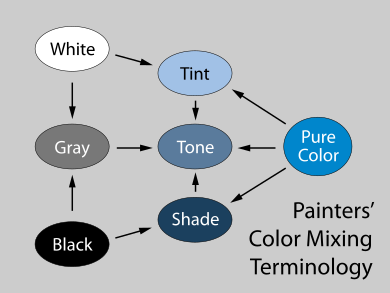
\includegraphics[width=40mm]{Tint-tone-shade}
		\column{.6\textwidth}
		\begin{exampleblock}{Examples of my posters}
			\href{run:./posters/portraitA1_rusltc.pdf}{\beamerbutton{styled portrait A1}} \\
			\href{run:./posters/landscape_oracy.pdf}{\beamerbutton{default landscape}}
			
			\begin{itemize}
				\item \alert{Beamer Button!}
				\verb|\href{URL}{\beamerbutton{text}}|
			\end{itemize}
		
		\end{exampleblock}
	\end{columns}
	
	
\end{enumerate}
\end{frame}

\begin{frame}[fragile=singleslide]{Adapt a .sty to produce a recognizable style}
	
	\textbf{Naming conventions:}
	
	beamerthemeLLT-poster.sty $\rightarrow$ beamerthemeMAK-poster.sty \\
	
	\verb|\usetheme{LLT-poster}|
	
	beamercolorthemeConspicuousCreep.sty \\
	
	\verb|\usecolortheme{ConspicuousCreep}|
	
	\bigskip
	
	\textbf{Use your own parameters for any elements of a template}
	
	\begin{itemize}
		\item headline/footline
		\item lower separation line head
		\item fonts, distances, width of lines
	\end{itemize}

	\textbf{Examples of definitions}
	\begin{lstlisting}[frame=single]
\setbeamercolor{structure}{fg=HazySummerEve}
\setbeamercolor{palette primary}{fg=black,bg=WinterSkin}
\setbeamercolor{foot}{bg=HazySummerEve!80,fg=white}
\setbeamercolor{enumerate item}{fg=Zen}
	\end{lstlisting}

\end{frame}

\begin{frame}[fragile]{Absolute positioning on page/frame and more on boxes}
	
\vspace{-2.3cm}
	
\begin{columns}[t]
	\column{.5\textwidth}
	\begin{block}{Positioning}
		\begin{enumerate}
			\item activate \verb|eso-pic| in preamble to get the grid
			\item create a \verb|textblock| env with \{width\} and (x,y) coordinates
			\item add contents, see e.g. $\rightarrow$
		\end{enumerate}
	\end{block}
	\column{.5\textwidth}
		\begin{block}{Frames around content}
		\begin{itemize}
			\item \verb|\begin{equation*}|
			\item a minipage env with width argument \verb|{13em}| inside a \verb|\fbox{}|
			\item \href{https://en.wikibooks.org/wiki/LaTeX/Boxes}{\underline{a plethora} of other options}
		\end{itemize}
	\end{block}
\end{columns}

\medskip

\alert{EXAMPLES:}

\begin{textblock*}{10pt}(10pt,180pt)
	\small
	\begin{equation*}  % starred vertion means no numbering
	\mathbf {H} = \frac{1}{2}\left( - \omega_{\mathrm{m}} + {\color{red}\delta \lambda(x)} \cos 2\theta_{\mathrm{m}} \right) \sigma_3 - \frac{  {\color{red}\delta \lambda(x)}  }{2} \sin \theta_{\mathrm{m}} \sigma_1
	\end{equation*}
\end{textblock*}

\begin{textblock*}{10pt}(170pt,220pt)
	\fbox{\begin{minipage}{15em}
			\centering
			I am framed some multi-line text \\
			framed with \textbf{minipage} environment \\
			and the frame width is 15em
		\end{minipage}
	}
\end{textblock*}
\end{frame}

\begin{frame}[fragile]{Gentle introduction to referencing}
	
	\href{https://en.wikibooks.org/wiki/LaTeX/Bibliography_Management}{\beamerbutton{Bibliography Management}}
	
	\begin{itemize}
		\item LaTeX has built-in support for citing references (\verb|\begin{thebibliography}{99}|)
		\item It is more convenient to store bibliography records externally (in .bib files, containing dictionary-like records for publications)
		\item There are two major formats for, and tools to process, these databases: (older) BibTeX and BibLaTex. 
		\item BibTeX and BibLaTex expect different keys in these dictionaries (year=\{2020\} vs date=\{2020\}). They are automatically mutually convertible\footnote{See Tharindu's solution}. 
		\item This workshop uses BibTeX.
	\end{itemize}
	
\end{frame}

\section[]{Task 5}

\begin{frame}[shrink=1]{Task 5. Make a presentation about one of your hobbies}
	\begin{tcolorbox}[width=\textwidth, colback={yellow!40!white}, title={Produce slides presenting your favourite pastime \\(maybe a book you read last). Try to use the following:}, colbacktitle=yellow!60!white, coltitle=black]
		\begin{itemize}
			\item a title slide with two logos
			\item ToC and progress before each section
			\item columns
			\item pictures
			\item alerted text
			\item overlays and incremental material presentation
			\item list environments
			\item boxes
			\item navigation symbols (at least the slides counter)
			\item references
		\end{itemize}
	Do you think you have time to develop your own unique presentation style file that would make all your talks stand out? 
	\end{tcolorbox}%
\end{frame}

\section[]{ToC-only References}

\begin{frame}{Embedded bibliography}
	\begin{thebibliography}{99}
		  \bibitem[\protect\citename{Akmajian and Lehrer, }1976]{akm76}
		Akmajian \& Lehrer A. 1976. NP-like quantifiers and the
		problem of determining the head of an NP. {\it Linguistic
			Analysis\/} {2}, 295--313.
		\bibitem[\protect\citename{Huddleston, }1984]{hud84}
		Huddleston, Rodney. 1984. {\it Introduction to the Grammar of
			English}. Cambridge: Cambridge University Press.
	\end{thebibliography}
\end{frame}

\begin{frame}[allowframebreaks,noframenumbering]{Bibliography (everything from file)}
	(from an external database)
	\nocite{*}
%	\bibliographystyle{apalike}
%	\bibliography{7_NLP-tasks-complexity}
\printbibliography
%\printbibliography[heading=none, title={Conference Proceedings}, type=inproceedings]
\end{frame}

\end{document}